\section{Requisitos funcionales}


\subsection{Diagramas de casos de uso}
Enseguida se presentaran los diagramas de caso de uso propuestos hasta la fecha

\begin{figure}[H]
	\centering
	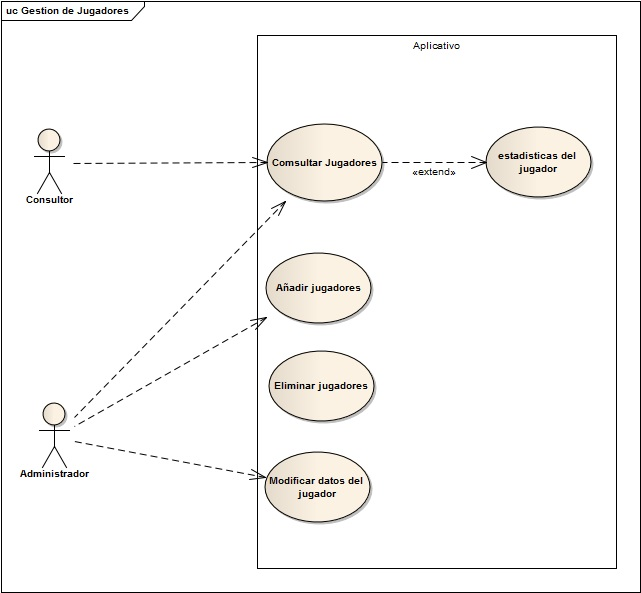
\includegraphics[width=0.8\linewidth]{Designe/imgs/gestionJ}
	\caption{Diagrama de casos de uso: Gestión de jugadores}
	\label{fig:gestionj}
\end{figure}

\begin{figure}[H]
	\centering
	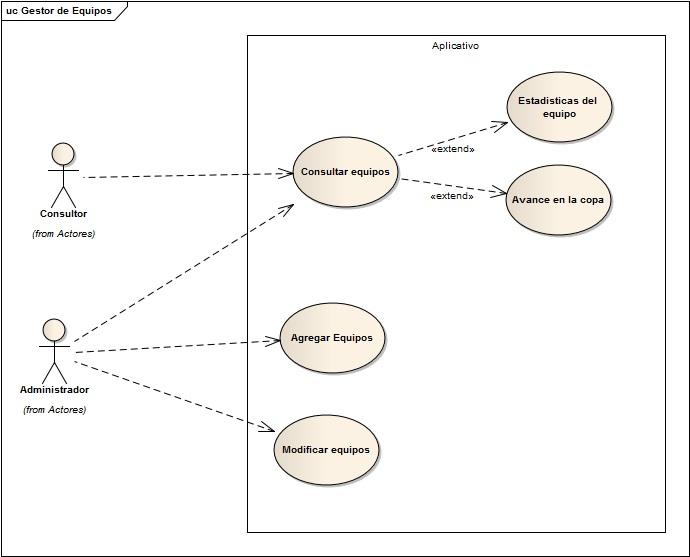
\includegraphics[width=0.8\linewidth]{Designe/imgs/gestionE}
	\caption{Diagrama de casos de uso: Gestión de equipos}
	\label{fig:gestionE}
\end{figure}

\begin{figure}[H]
	\centering
	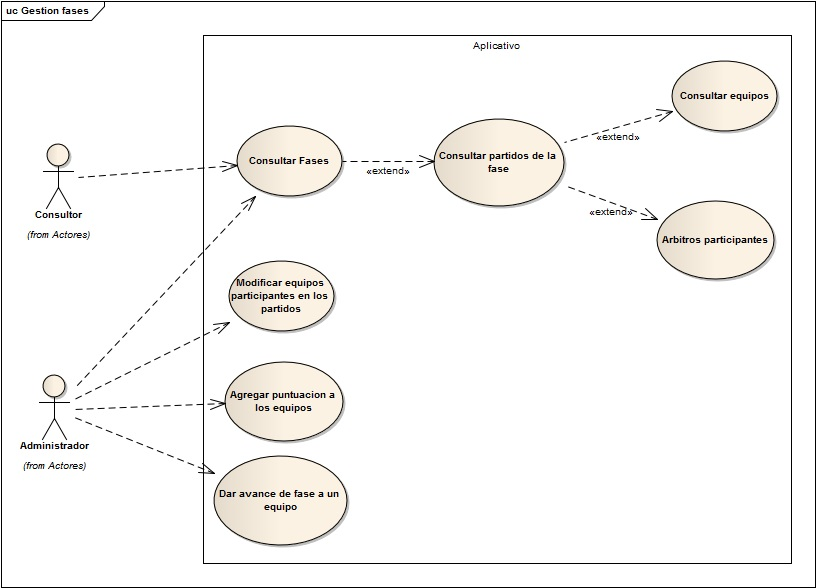
\includegraphics[width=0.8\linewidth]{Designe/imgs/gestionF}
	\caption{Diagrama de casos de uso: Gestión de Fases}
	\label{fig:gestionF}
\end{figure}


%-------------------------------------------------
%_--------------------------------------------------


\subsection{Definición de actores}
 
 
 
\begin{table}[H]
	\centering
	\caption{ACT-01}
	\label{ACT-01}
	\begin{tabular}{|l|l|}
		\hline
		\textbf{ACT-01}      & \textbf{Consultor}                                 \\ \hline
		\textbf{Version}     & 1                                                  \\ \hline
		\textbf{Autores}     & Edwar Diaz Ruiz                                    \\ \hline
		\textbf{Fuentes}     & Universidad Distrital Francisco Josec de Caldas    \\ \hline
		\textbf{Descripcion} & es la persona que ve los resultados y estadisticas \\ \hline
		\textbf{comentarios} & ninguno             \\ \hline
	\end{tabular}
\end{table}

\begin{table}[H]
	\centering
	\caption{ACT-02}
	\label{ACT-02}
	\begin{tabular}{|l|l|}
		\hline
		\textbf{ACT-02}      & \textbf{Administrador}                                 \\ \hline
		\textbf{Version}     & 1                                                  \\ \hline
		\textbf{Autores}     & Edwar Diaz Ruiz                                    \\ \hline
		\textbf{Fuentes}     & Universidad Distrital Francisco Josec de Caldas    \\ \hline
		\textbf{Descripcion} &  {\begin{tabular}[c]{@{}l@{}}es el administrador de la base de datos\end{tabular}} \\ \hline
		\textbf{comentarios} & ninguno             \\ \hline
	\end{tabular}
\end{table}


\subsection{Casos de uso del sistema}

Se han de definir los requisitos funcionales del sistema de manera detallada.

\begin{table}[H]
	\centering
	\caption{RF-01}
	\label{RF-01}
	\begin{tabular}{|l|l|l|}
		\hline
		\textbf{RF-01}                             & \multicolumn{2}{l|}{\textbf{Consultar jugadores}}         \\ \hline
		\textbf{Version}                           & \multicolumn{2}{l|}{1}                  \\ \hline
		\textbf{Autores}                           & \multicolumn{2}{l|}{Edwar Diaz Ruiz}    \\ \hline
		\textbf{Fuentes}                           & \multicolumn{2}{l|}{f}                  \\ \hline
		\textbf{Objetivos Asociados}               & \multicolumn{2}{l|}{OBJ-03}                  \\ \hline
		\textbf{Requisitos Asociados}              & \multicolumn{2}{l|}{RI-01}                  \\ \hline
		\textbf{Descripcion}                       & \multicolumn{2}{l|} {\begin{tabular}[c]{@{}l@{}}sea el consultor o el administrador\\ estos podrán ver la informacion \\ de los jugadores\end{tabular}}                  \\ \hline
		\textbf{Precondicion}                      & \multicolumn{2}{l|}{ninguna}                  \\ \hline
		\multirow{4}{*}{\textbf{Secuandia normal}} & \textbf{Paso} & \textbf{Accion}         \\ \cline{2-3} 
		& 1            &  {\begin{tabular}[c]{@{}l@{}}el usuario seleccionara la \\búsqueda de jugadores \end{tabular}}                      \\ \cline{2-3} 
		& 2            & {\begin{tabular}[c]{@{}l@{}}luego buscara a su jugador de \\ interés ya sea por el nombre, su equipo \\ o algún otro parámetro de búsqueda \\ disponible \end{tabular}}                        \\ \cline{2-3} 
		& 3            & {\begin{tabular}[c]{@{}l@{}}el sistema filtra la lista de jugadores\\ según los parámetros determinados\\ para la búsqueda.  \end{tabular}} 
		 \\ \cline{2-3} 
		& 4            & {\begin{tabular}[c]{@{}l@{}}el usuario selecciona al jugador\\ del cual desee saber la obtener \\la información.  \end{tabular}}
		 \\ \cline{2-3} 
		& 5            & {\begin{tabular}[c]{@{}l@{}}el sistema realiza la consulta\\ para respectiva a la base de datos.  \end{tabular}}
		 \\ \cline{2-3} 
		& 6            & {\begin{tabular}[c]{@{}l@{}}el sistema obtiene la información\\ respectiva y la muestra al usuario.  \end{tabular}}                      \\ \hline
		\textbf{PostCondicion}                     & \multicolumn{2}{l|}{PD}                 \\ \hline
	%	\multirow{3}{*}{\textbf{excepciones}}      & \textbf{paso} & \textbf{accion}         \\ \cline{2-3} 
	%	& p1            & sd                      \\ \cline{2-3} 
	%	& p2            & sd                      \\ \hline
	%	\multirow{3}{*}{\textbf{rendimiento}}      & \textbf{paso} & \textbf{cota de tiempo} \\ \cline{2-3} 
	%	& q             & sd                      \\ \cline{2-3} 
	%	& q2            & sd                      \\ \hline
		\textbf{frecuencia esperada}               & \multicolumn{2}{l|}{eventual}                 \\ \hline
		\textbf{importancia}                       & \multicolumn{2}{l|}{media}                 \\ \hline
		\textbf{urgencia}                          & \multicolumn{2}{l|}{media}                 \\ \hline
		%\textbf{estados}                           & %\multicolumn{2}{l|}{sd}                 \\ \hline
		%\textbf{estabilidad}                       & \multicolumn{2}{l|}{sd}                 \\ \hline
		\textbf{comentarios}                       & \multicolumn{2}{l|}{ninguno}                 \\ \hline
	\end{tabular}
\end{table}

\begin{table}[H]
	\centering
	\caption{RF-02}
	\label{RF-02}
	\begin{tabular}{|l|l|l|}
		\hline
		\textbf{RF-02}                             & \multicolumn{2}{l|}{\textbf{Consultar estadisticas de los jugadores}}         \\ \hline
		\textbf{Version}                           & \multicolumn{2}{l|}{1}                  \\ \hline
		\textbf{Autores}                           & \multicolumn{2}{l|}{Edwar Diaz Ruiz}    \\ \hline
		\textbf{Fuentes}                           & \multicolumn{2}{l|}{f}                  \\ \hline
		\textbf{Objetivos Asociados}               & \multicolumn{2}{l|}{OBJ-03}                  \\ \hline
		\textbf{Requisitos Asociados}              & \multicolumn{2}{l|}{RI-01}                  \\ \hline
		\textbf{Descripcion}                       & \multicolumn{2}{l|} {\begin{tabular}[c]{@{}l@{}}se mostraran estadisticas de los jugadores\end{tabular}}                  \\ \hline
		\textbf{Precondicion}                      & \multicolumn{2}{l|}{RF-01}                  \\ \hline
		\multirow{4}{*}{\textbf{Secuandia normal}} & \textbf{Paso} & \textbf{Accion}         \\ \cline{2-3} 
		& 1            &  {\begin{tabular}[c]{@{}l@{}}el usuario seleccionara la opción\\ de mostrar estadisticas \end{tabular}}                      \\ \cline{2-3} 
		& 2            & {\begin{tabular}[c]{@{}l@{}}el sistema hará la consulta para obtener las estadisticas \end{tabular}}                        \\ \cline{2-3} 
		& 3            & {\begin{tabular}[c]{@{}l@{}}el sistema obtendrá las estadisticas\\ y las mostrara al usuario \end{tabular}} 
		\\ \hline
		\textbf{PostCondicion}                     & \multicolumn{2}{l|}{PD}                 \\ \hline
		%	\multirow{3}{*}{\textbf{excepciones}}      & \textbf{paso} & \textbf{accion}         \\ \cline{2-3} 
		%	& p1            & sd                      \\ \cline{2-3} 
		%	& p2            & sd                      \\ \hline
		%	\multirow{3}{*}{\textbf{rendimiento}}      & \textbf{paso} & \textbf{cota de tiempo} \\ \cline{2-3} 
		%	& q             & sd                      \\ \cline{2-3} 
		%	& q2            & sd                      \\ \hline
		\textbf{frecuencia esperada}               & \multicolumn{2}{l|}{eventual}                 \\ \hline
		\textbf{importancia}                       & \multicolumn{2}{l|}{media}                 \\ \hline
		\textbf{urgencia}                          & \multicolumn{2}{l|}{media}                 \\ \hline
		%\textbf{estados}                           & %\multicolumn{2}{l|}{sd}                 \\ \hline
		%\textbf{estabilidad}                       & \multicolumn{2}{l|}{sd}                 \\ \hline
		\textbf{comentarios}                       & \multicolumn{2}{l|}{ninguno}                 \\ \hline
	\end{tabular}
\end{table}
